%% bare_conf.tex
%% V1.3
%% 2007/01/11
%% by Michael Shell
%% See:
%% http://www.michaelshell.org/
%% for current contact information.
%%
%% This is a skeleton file demonstrating the use of IEEEtran.cls
%% (requires IEEEtran.cls version 1.7 or later) with an IEEE conference paper.
%%
%% Support sites:
%% http://www.michaelshell.org/tex/ieeetran/
%% http://www.ctan.org/tex-archive/macros/latex/contrib/IEEEtran/
%% and
%% http://www.ieee.org/

%%*************************************************************************
%% Legal Notice:
%% This code is offered as-is without any warranty either expressed or
%% implied; without even the implied warranty of MERCHANTABILITY or
%% FITNESS FOR A PARTICULAR PURPOSE! 
%% User assumes all risk.
%% In no event shall IEEE or any contributor to this code be liable for
%% any damages or losses, including, but not limited to, incidental,
%% consequential, or any other damages, resulting from the use or misuse
%% of any information contained here.
%%
%% All comments are the opinions of their respective authors and are not
%% necessarily endorsed by the IEEE.
%%
%% This work is distributed under the LaTeX Project Public License (LPPL)
%% ( http://www.latex-project.org/ ) version 1.3, and may be freely used,
%% distributed and modified. A copy of the LPPL, version 1.3, is included
%% in the base LaTeX documentation of all distributions of LaTeX released
%% 2003/12/01 or later.
%% Retain all contribution notices and credits.
%% ** Modified files should be clearly indicated as such, including  **
%% ** renaming them and changing author support contact information. **
%%
%% File list of work: IEEEtran.cls, IEEEtran_HOWTO.pdf, bare_adv.tex,
%%                    bare_conf.tex, bare_jrnl.tex, bare_jrnl_compsoc.tex
%%*************************************************************************

% *** Authors should verify (and, if needed, correct) their LaTeX system  ***
% *** with the testflow diagnostic prior to trusting their LaTeX platform ***
% *** with production work. IEEE's font choices can trigger bugs that do  ***
% *** not appear when using other class files.                            ***
% The testflow support page is at:
% http://www.michaelshell.org/tex/testflow/



% Note that the a4paper option is mainly intended so that authors in
% countries using A4 can easily print to A4 and see how their papers will
% look in print - the typesetting of the document will not typically be
% affected with changes in paper size (but the bottom and side margins will).
% Use the testflow package mentioned above to verify correct handling of
% both paper sizes by the user's LaTeX system.
%
% Also note that the "draftcls" or "draftclsnofoot", not "draft", option
% should be used if it is desired that the figures are to be displayed in
% draft mode.
%
\documentclass[conference]{IEEEtran}
% Add the compsoc option for Computer Society conferences.
%
% If IEEEtran.cls has not been installed into the LaTeX system files,
% manually specify the path to it like:
% \documentclass[conference]{../sty/IEEEtran}





% Some very useful LaTeX packages include:
% (uncomment the ones you want to load)


% *** MISC UTILITY PACKAGES ***
%
%\usepackage{ifpdf}
% Heiko Oberdiek's ifpdf.sty is very useful if you need conditional
% compilation based on whether the output is pdf or dvi.
% usage:
% \ifpdf
%   % pdf code
% \else
%   % dvi code
% \fi
% The latest version of ifpdf.sty can be obtained from:
% http://www.ctan.org/tex-archive/macros/latex/contrib/oberdiek/
% Also, note that IEEEtran.cls V1.7 and later provides a builtin
% \ifCLASSINFOpdf conditional that works the same way.
% When switching from latex to pdflatex and vice-versa, the compiler may
% have to be run twice to clear warning/error messages.






% *** CITATION PACKAGES ***
%
%\usepackage{cite}
% cite.sty was written by Donald Arseneau
% V1.6 and later of IEEEtran pre-defines the format of the cite.sty package
% \cite{} output to follow that of IEEE. Loading the cite package will
% result in citation numbers being automatically sorted and properly
% "compressed/ranged". e.g., [1], [9], [2], [7], [5], [6] without using
% cite.sty will become [1], [2], [5]--[7], [9] using cite.sty. cite.sty's
% \cite will automatically add leading space, if needed. Use cite.sty's
% noadjust option (cite.sty V3.8 and later) if you want to turn this off.
% cite.sty is already installed on most LaTeX systems. Be sure and use
% version 4.0 (2003-05-27) and later if using hyperref.sty. cite.sty does
% not currently provide for hyperlinked citations.
% The latest version can be obtained at:
% http://www.ctan.org/tex-archive/macros/latex/contrib/cite/
% The documentation is contained in the cite.sty file itself.






% *** GRAPHICS RELATED PACKAGES ***
%
\ifCLASSINFOpdf
   \usepackage[pdftex]{graphicx}
  % declare the path(s) where your graphic files are
  % \graphicspath{{../pdf/}{../jpeg/}}
  % and their extensions so you won't have to specify these with
  % every instance of \includegraphics
  % \DeclareGraphicsExtensions{.pdf,.jpeg,.png}
\else
  % or other class option (dvipsone, dvipdf, if not using dvips). graphicx
  % will default to the driver specified in the system graphics.cfg if no
  % driver is specified.
   \usepackage[dvips]{graphicx}
  % declare the path(s) where your graphic files are
  % \graphicspath{{../eps/}}
  % and their extensions so you won't have to specify these with
  % every instance of \includegraphics
  % \DeclareGraphicsExtensions{.eps}
\fi
% graphicx was written by David Carlisle and Sebastian Rahtz. It is
% required if you want graphics, photos, etc. graphicx.sty is already
% installed on most LaTeX systems. The latest version and documentation can
% be obtained at: 
% http://www.ctan.org/tex-archive/macros/latex/required/graphics/
% Another good source of documentation is "Using Imported Graphics in
% LaTeX2e" by Keith Reckdahl which can be found as epslatex.ps or
% epslatex.pdf at: http://www.ctan.org/tex-archive/info/
%
% latex, and pdflatex in dvi mode, support graphics in encapsulated
% postscript (.eps) format. pdflatex in pdf mode supports graphics
% in .pdf, .jpeg, .png and .mps (metapost) formats. Users should ensure
% that all non-photo figures use a vector format (.eps, .pdf, .mps) and
% not a bitmapped formats (.jpeg, .png). IEEE frowns on bitmapped formats
% which can result in "jaggedy"/blurry rendering of lines and letters as
% well as large increases in file sizes.
%
% You can find documentation about the pdfTeX application at:
% http://www.tug.org/applications/pdftex





% *** MATH PACKAGES ***
%
%\usepackage[cmex10]{amsmath}
% A popular package from the American Mathematical Society that provides
% many useful and powerful commands for dealing with mathematics. If using
% it, be sure to load this package with the cmex10 option to ensure that
% only type 1 fonts will utilized at all point sizes. Without this option,
% it is possible that some math symbols, particularly those within
% footnotes, will be rendered in bitmap form which will result in a
% document that can not be IEEE Xplore compliant!
%
% Also, note that the amsmath package sets \interdisplaylinepenalty to 10000
% thus preventing page breaks from occurring within multiline equations. Use:
%\interdisplaylinepenalty=2500
% after loading amsmath to restore such page breaks as IEEEtran.cls normally
% does. amsmath.sty is already installed on most LaTeX systems. The latest
% version and documentation can be obtained at:
% http://www.ctan.org/tex-archive/macros/latex/required/amslatex/math/





% *** SPECIALIZED LIST PACKAGES ***
%
%\usepackage{algorithmic}
% algorithmic.sty was written by Peter Williams and Rogerio Brito.
% This package provides an algorithmic environment fo describing algorithms.
% You can use the algorithmic environment in-text or within a figure
% environment to provide for a floating algorithm. Do NOT use the algorithm
% floating environment provided by algorithm.sty (by the same authors) or
% algorithm2e.sty (by Christophe Fiorio) as IEEE does not use dedicated
% algorithm float types and packages that provide these will not provide
% correct IEEE style captions. The latest version and documentation of
% algorithmic.sty can be obtained at:
% http://www.ctan.org/tex-archive/macros/latex/contrib/algorithms/
% There is also a support site at:
% http://algorithms.berlios.de/index.html
% Also of interest may be the (relatively newer and more customizable)
% algorithmicx.sty package by Szasz Janos:
% http://www.ctan.org/tex-archive/macros/latex/contrib/algorithmicx/




% *** ALIGNMENT PACKAGES ***
%
%\usepackage{array}
% Frank Mittelbach's and David Carlisle's array.sty patches and improves
% the standard LaTeX2e array and tabular environments to provide better
% appearance and additional user controls. As the default LaTeX2e table
% generation code is lacking to the point of almost being broken with
% respect to the quality of the end results, all users are strongly
% advised to use an enhanced (at the very least that provided by array.sty)
% set of table tools. array.sty is already installed on most systems. The
% latest version and documentation can be obtained at:
% http://www.ctan.org/tex-archive/macros/latex/required/tools/


%\usepackage{mdwmath}
%\usepackage{mdwtab}
% Also highly recommended is Mark Wooding's extremely powerful MDW tools,
% especially mdwmath.sty and mdwtab.sty which are used to format equations
% and tables, respectively. The MDWtools set is already installed on most
% LaTeX systems. The lastest version and documentation is available at:
% http://www.ctan.org/tex-archive/macros/latex/contrib/mdwtools/


% IEEEtran contains the IEEEeqnarray family of commands that can be used to
% generate multiline equations as well as matrices, tables, etc., of high
% quality.


%\usepackage{eqparbox}
% Also of notable interest is Scott Pakin's eqparbox package for creating
% (automatically sized) equal width boxes - aka "natural width parboxes".
% Available at:
% http://www.ctan.org/tex-archive/macros/latex/contrib/eqparbox/





% *** SUBFIGURE PACKAGES ***
%\usepackage[tight,footnotesize]{subfigure}
% subfigure.sty was written by Steven Douglas Cochran. This package makes it
% easy to put subfigures in your figures. e.g., "Figure 1a and 1b". For IEEE
% work, it is a good idea to load it with the tight package option to reduce
% the amount of white space around the subfigures. subfigure.sty is already
% installed on most LaTeX systems. The latest version and documentation can
% be obtained at:
% http://www.ctan.org/tex-archive/obsolete/macros/latex/contrib/subfigure/
% subfigure.sty has been superceeded by subfig.sty.



%\usepackage[caption=false]{caption}
%\usepackage[font=footnotesize]{subfig}
% subfig.sty, also written by Steven Douglas Cochran, is the modern
% replacement for subfigure.sty. However, subfig.sty requires and
% automatically loads Axel Sommerfeldt's caption.sty which will override
% IEEEtran.cls handling of captions and this will result in nonIEEE style
% figure/table captions. To prevent this problem, be sure and preload
% caption.sty with its "caption=false" package option. This is will preserve
% IEEEtran.cls handing of captions. Version 1.3 (2005/06/28) and later 
% (recommended due to many improvements over 1.2) of subfig.sty supports
% the caption=false option directly:
%\usepackage[caption=false,font=footnotesize]{subfig}
%
% The latest version and documentation can be obtained at:
% http://www.ctan.org/tex-archive/macros/latex/contrib/subfig/
% The latest version and documentation of caption.sty can be obtained at:
% http://www.ctan.org/tex-archive/macros/latex/contrib/caption/




% *** FLOAT PACKAGES ***
%
%\usepackage{fixltx2e}
% fixltx2e, the successor to the earlier fix2col.sty, was written by
% Frank Mittelbach and David Carlisle. This package corrects a few problems
% in the LaTeX2e kernel, the most notable of which is that in current
% LaTeX2e releases, the ordering of single and double column floats is not
% guaranteed to be preserved. Thus, an unpatched LaTeX2e can allow a
% single column figure to be placed prior to an earlier double column
% figure. The latest version and documentation can be found at:
% http://www.ctan.org/tex-archive/macros/latex/base/



%\usepackage{stfloats}
% stfloats.sty was written by Sigitas Tolusis. This package gives LaTeX2e
% the ability to do double column floats at the bottom of the page as well
% as the top. (e.g., "\begin{figure*}[!b]" is not normally possible in
% LaTeX2e). It also provides a command:
%\fnbelowfloat
% to enable the placement of footnotes below bottom floats (the standard
% LaTeX2e kernel puts them above bottom floats). This is an invasive package
% which rewrites many portions of the LaTeX2e float routines. It may not work
% with other packages that modify the LaTeX2e float routines. The latest
% version and documentation can be obtained at:
% http://www.ctan.org/tex-archive/macros/latex/contrib/sttools/
% Documentation is contained in the stfloats.sty comments as well as in the
% presfull.pdf file. Do not use the stfloats baselinefloat ability as IEEE
% does not allow \baselineskip to stretch. Authors submitting work to the
% IEEE should note that IEEE rarely uses double column equations and
% that authors should try to avoid such use. Do not be tempted to use the
% cuted.sty or midfloat.sty packages (also by Sigitas Tolusis) as IEEE does
% not format its papers in such ways.





% *** PDF, URL AND HYPERLINK PACKAGES ***
%
%\usepackage{url}
% url.sty was written by Donald Arseneau. It provides better support for
% handling and breaking URLs. url.sty is already installed on most LaTeX
% systems. The latest version can be obtained at:
% http://www.ctan.org/tex-archive/macros/latex/contrib/misc/
% Read the url.sty source comments for usage information. Basically,
% \url{my_url_here}.


% *** Do not adjust lengths that control margins, column widths, etc. ***
% *** Do not use packages that alter fonts (such as pslatex).         ***
% There should be no need to do such things with IEEEtran.cls V1.6 and later.
% (Unless specifically asked to do so by the journal or conference you plan
% to submit to, of course. )


% correct bad hyphenation here
\hyphenation{op-tical net-works semi-conduc-tor}


\begin{document}
%
% paper title
% can use linebreaks \\ within to get better formatting as desired
\title{``How is your community doing?'' studying snapshots of development communities}


% author names and affiliations
% use a multiple column layout for up to three different
% affiliations
\author{\IEEEauthorblockN{Damian A. Tamburri\\ Patricia Lago\\ and Hans Van Vliet}
\IEEEauthorblockA{Department of\\ Computer Science\\
VU University Amsterdam, The Netherlands\\
$[$d.a.tamburri, p.lago, j.c.van.vliet$]$@vu.nl}
\and
\IEEEauthorblockN{Martin von Weissenberg}
\IEEEauthorblockA{Hanken
School of Economics\\
Department of Information Systems\\
Helsinki, Finland \\
martin.vonweissenberg@hanken.fi }}

% conference papers do not typically use \thanks and this command
% is locked out in conference mode. If really needed, such as for
% the acknowledgment of grants, issue a \IEEEoverridecommandlockouts
% after \documentclass

% for over three affiliations, or if they all won't fit within the width
% of the page, use this alternative format:
% 
%\author{\IEEEauthorblockN{Michael Shell\IEEEauthorrefmark{1},
%Homer Simpson\IEEEauthorrefmark{2},
%James Kirk\IEEEauthorrefmark{3}, 
%Montgomery Scott\IEEEauthorrefmark{3} and
%Eldon Tyrell\IEEEauthorrefmark{4}}
%\IEEEauthorblockA{\IEEEauthorrefmark{1}School of Electrical and Computer Engineering\\
%Georgia Institute of Technology,
%Atlanta, Georgia 30332--0250\\ Email: see http://www.michaelshell.org/contact.html}
%\IEEEauthorblockA{\IEEEauthorrefmark{2}Twentieth Century Fox, Springfield, USA\\
%Email: homer@thesimpsons.com}
%\IEEEauthorblockA{\IEEEauthorrefmark{3}Starfleet Academy, San Francisco, California 96678-2391\\
%Telephone: (800) 555--1212, Fax: (888) 555--1212}
%\IEEEauthorblockA{\IEEEauthorrefmark{4}Tyrell Inc., 123 Replicant Street, Los Angeles, California 90210--4321}}




% use for special paper notices
%\IEEEspecialpapernotice{(Invited Paper)}




% make the title area
\maketitle


\begin{abstract}
%\boldmath
Engineering software is a social activity. Software projects' success is very often dependent on how the welfare of their development community. This connection becomes especially delicate when multiple communities have to join forces (e.g. in global software engineering). So far however, software engineering discipline lacks systematic methods to steer development communities. In this paper we present a method to study development communities. We elaborated the method conducting a real-life case-study in a large software development organisation. 
One key finding is that observable organisational information misleads community detection. In addition, in the case-study we found many organisational barriers, both negative and positive ones. 
%If they are, they can be tackled by analysing the status of the software development community. We illustrate with a case-study.
%, by making its key attributes explicit. In addition, we suggest ways in which practitioners can use the community state, to adjust the relative communities (e.g. by adding specific technologies or changing organisational goals). 
\end{abstract}
% IEEEtran.cls defaults to using nonbold math in the Abstract.
% This preserves the distinction between vectors and scalars. However,
% if the conference you are submitting to favors bold math in the abstract,
% then you can use LaTeX's standard command \boldmath at the very start
% of the abstract to achieve this. Many IEEE journals/conferences frown on
% math in the abstract anyway.

% no keywords

% For peer review papers, you can put extra information on the cover
% page as needed:
% \ifCLASSOPTIONpeerreview
% \begin{center} \bfseries EDICS Category: 3-BBND \end{center}
% \fi
%
% For peerreview papers, this IEEEtran command inserts a page break and
% creates the second title. It will be ignored for other modes.
\IEEEpeerreviewmaketitle

\section{Introduction}

The craft of software is becoming more and more a social activity \cite{specissue}. Several studies suggest that engineers spend between 70 and 85\% of their time working with other people (e.g. end-user focus groups, managers, business sponsors, etc.) \cite{socialbook}. This means that in 70-85\% of times, software engineering success is a community effort, rather than a success of single individuals. This figure becomes critical with the increase of diversity and size of the development community. For example, Global Software Engineering (GSE) is a development strategy entailing global teams to collaborate together from different locations in different timezones \cite{gsdbook}. In this circumstance, distances in time, space and culture, magnify project risks connected to failures in the development social structure \cite{empirglob,nachiappan,icgseoss}.
The problem persists since software practitioners lack a systematic method to study (global) development social structures. In previous work \cite{specissue} we provided a mechanism to uncover social communities latent in software development but we learned that it shows many limitations when used in real-life scenarios.
%As a consequence, there is no way for software engineering practitioners to effectively act upon the development community they are part of.
To tackle this issue we conducted a real-life case-study in a big software development organisation. 

The study resulted in a semi-automatic method to snapshot a development community. The method uses a questionnaire to gather necessary information about the observed community. Finally, the method uses a decision-tree \cite{specissue} to interpret the information in the questionnaire. 
 
We made three observations: (a) the method helps uncovering the status of development communities but it cannot be fully automated; (b) the method makes it possible to uncover organisational barriers; (c) the community snapshot can have a limited number of possible forms, each with its own particular characteristics, these forms are worthy of further study since they could act as proxies for quality of the observed community.
%In addition we suggest ways to manipulate the community state, e.g. to change community type or its focus. 
%In algorithms theory, a process state is given by the (current) values of all variables within the scope of the process \cite{algos}.
%Our method is based on empirical evidence. 

%%%%%%%%%% NOOOOOO!!!
%We found that a \emph{social community} is a specific type of social network for which certain attributes remain constantly true.

%We found that the status of a community is given by a set of paths on a community decision-tree.
%For example, imagine you are working within a UK open-source forge that collaborates with another open-source community from the US. This basic information conveys two critical informations: (a) the resulting community (US+UK) is \emph{dispersed}, i.e. not collocated; (b) the resulting community is \emph{informal}. According to \cite{ossslr,specissue} the presence of these two attributes is necessary and sufficient to identify an \emph{Informal Network} social community type.
%

%Finally, we compare the identified social community attributes (i.e. the community state) with empirical results from previous work \cite{ossslr}. This last step allows us to understand what can be done to improve the communities, e.g. by encouraging changes in attributes.
%The benefits of using our method are threefold: first, practitioners can use the questionnaire as a checklist for missing management information; second, the questionnaire can be used as a guideline to engineer communities for a specific software development problem; third, the community state we obtain can be cross-referenced with development velocity to evaluate community effectiveness in the current state.
\begin{figure*}
\hspace{.5cm}
%\begin{sideways}
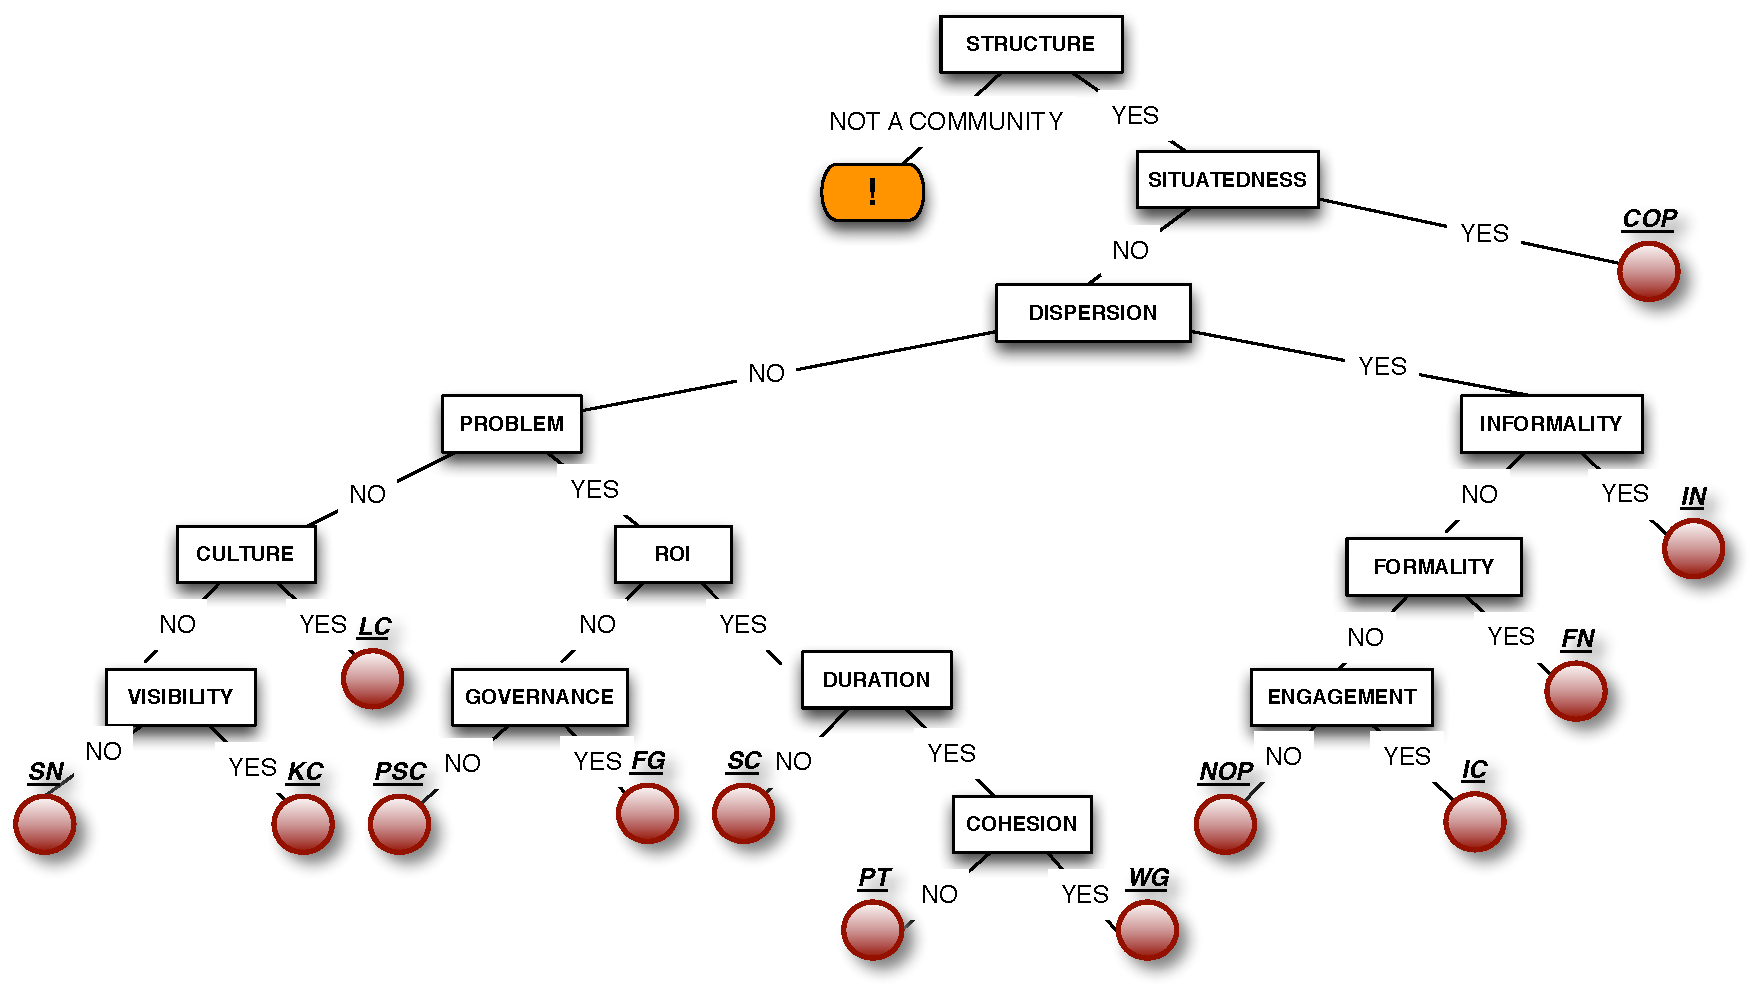
\includegraphics[width=6.3in]{tree}%
%\end{sideways}
\caption{a decision-tree to uncover social communities \cite{specissue}}\label{tree}
\end{figure*}

The rest of the paper is structured as follows: Section \ref{devcomm} provides some background on software engineering and the study of its social aspects; Sections \ref{rq} and \ref{mm} provides our research questions, evidence and methods; Section \ref{cs} presents the case-study we conducted; Section \ref{res} provides our results and discussion. Finally, Section \ref{conc} concludes the paper.

% no \IEEEPARstart
%This demo file is intended to serve as a ``starter file''
%for IEEE conference papers produced under \LaTeX\ using
%IEEEtran.cls version 1.7 and later.
%% You must have at least 2 lines in the paragraph with the drop letter
%% (should never be an issue)
%I wish you the best of success.
%\hfill mds

\section{Research Question}\label{rq}

The work presented in this paper was realised with the following research question:

\begin{center}
{\bf How can we snapshot software development communities?}
\end{center}

%\begin{itemize}
%\item explain impact of the question and importance of answering
%\end{itemize}
Providing an intelligible shape for an observable software development community is the first step towards steering community operations. For example, global software development literature acknowledged that global communication is compromised by the presence of organisational barriers within and between communities \cite{gse,gsdbook}. Studying snapshots of global communities could enable the development of ad-hoc governance models, that adapt based on current (or desired) community snapshots. In addition, studying snapshots of communities, managers can plot cross-community communication patterns that match exactly the current status. For example, during a Scrum sprint, Scrum coaches can evaluate snapshots of the development community to understand its productivity and adapt it as needed (e.g. to avoid ``Crunch-times'' in Scrum).


\section{Previous and Related work: On the Benefits of Studying and Supporting Software Development Communities}\label{devcomm}
%\begin{itemize}
%\item related work from socio-technical congruence
%\item related work dana damian
%%\item conway's law?
%\item other works in ged for social studies
%\item productivity and agile methods to be adopted in gsd
%\end{itemize}

Literature in GSE already recognises the need to study global communities. More in particular, many works such as \cite{nachiappan} have studied empirically the effect of organisational structures on the quality of software. These works motivate further studies to understand, represent and support social structures and communities. In addition, similar works such as \cite{uls,rel9} study the effect of socio-technical congruence on designing global systems as well as the process of global engineering. Such works suggests that understanding how coordination requirements map to their people counterpart is critical to steer information across global communities successfully. Our work is limited to identifying communities and finding ways to study their observable characteristics. 
Other works such as \cite{Davenport2001} study the impact of successful communities on socio-technical problems (e.g. coordination, shared understanding, etc.). These works take a more social and organisational approach, pointing out the paramount importance of supporting explicitly the work of communities rather than allocating tasks to single individuals. In previous work \cite{icgseoss,ossslr}, we found that observable \emph{social communities} captured in \cite{Davenport2001} are a composition of known social community types \cite{ossslr}.
Finally, works such as \cite{scrum} study the impact of agile methods on a large scale distributed software engineering attempt. Understanding the impact and changes on global communities forced in by agile methods adoption, could be a key advantage in using such methods successfully, especially on a global scale.
Our work in this paper does not explore the impact of organisational decisions affecting the community status, but introduces a method to understand the community by snapshotting its current status, e.g. to support related organisational decisions such as agile adoption.

%
%previous research in software engineering, organisational sciences and systems theory has observed many social community types. Over time, many attributes were observed and used to characterise these community. We analyse empirical evidence with the aim of pinpointing the attributes that are necessary and sufficient to capture the state of a certain community
%
%Second, {\bf how can we act on the status of a software development community?}  .\\
%
%Finally, {\bf how can practitioners use the state-of-the-art in social communities to improve development collaboration?}  .\\

% 
%\hfill January 11, 2007
%
%\subsection{Subsection Heading Here}
%Subsection text here.
%
%
%\subsubsection{Subsubsection Heading Here}
%Subsubsection text here.
%

\section{Methods and Empirical Evidence Used}\label{mm}
%This paper introduces a method to study a development community using a case-study. 
We carried out a case-study stemming from the theoretical foundations in previous work. More in particular, two researchers studied separately the empirical evidence and conducted the case-study in parallel with minimal interaction. The ``double'' case-study was used to ensure reliability of results. In addition, by conducting two of the same case-study in parallel we were able to confidently generalise some findings.

Both case-studies, and subsequently the findings, were coordinated and checked by two senior researchers.
%TODO: explain that two people conducted the case-study with the same material in parallel with minimal interaction on the case study, as overseen by two senior researchers. when it was finished the results were compared for evaluation. the method can be generalised since both researchers followed the same emergent path and encountered the same probs, that were solved in pretty much the same way.\\
%The following sections describe materials and methods in more detail.

%\begin{itemize}
%\item describe work in the SLR
%\item describe work in ICGSE paper
%\item describe work in IEEE Sw paper
%\item related work
%\end{itemize}
%
%\subsection{Materials Used}
The empirical evidence used in our work, stems from empirical research conducted in a big organisation, active in the mobile technologies market. The organisation (called Company X from now on) is multinational and employs over 50k people in more than 15 worldwide sites. At the time the empirical research was conducted, the organisation has a market revenue of over 5-7 billion euros. 
\begin{figure}[h!]
\hspace{-.2cm}
%\begin{sideways}
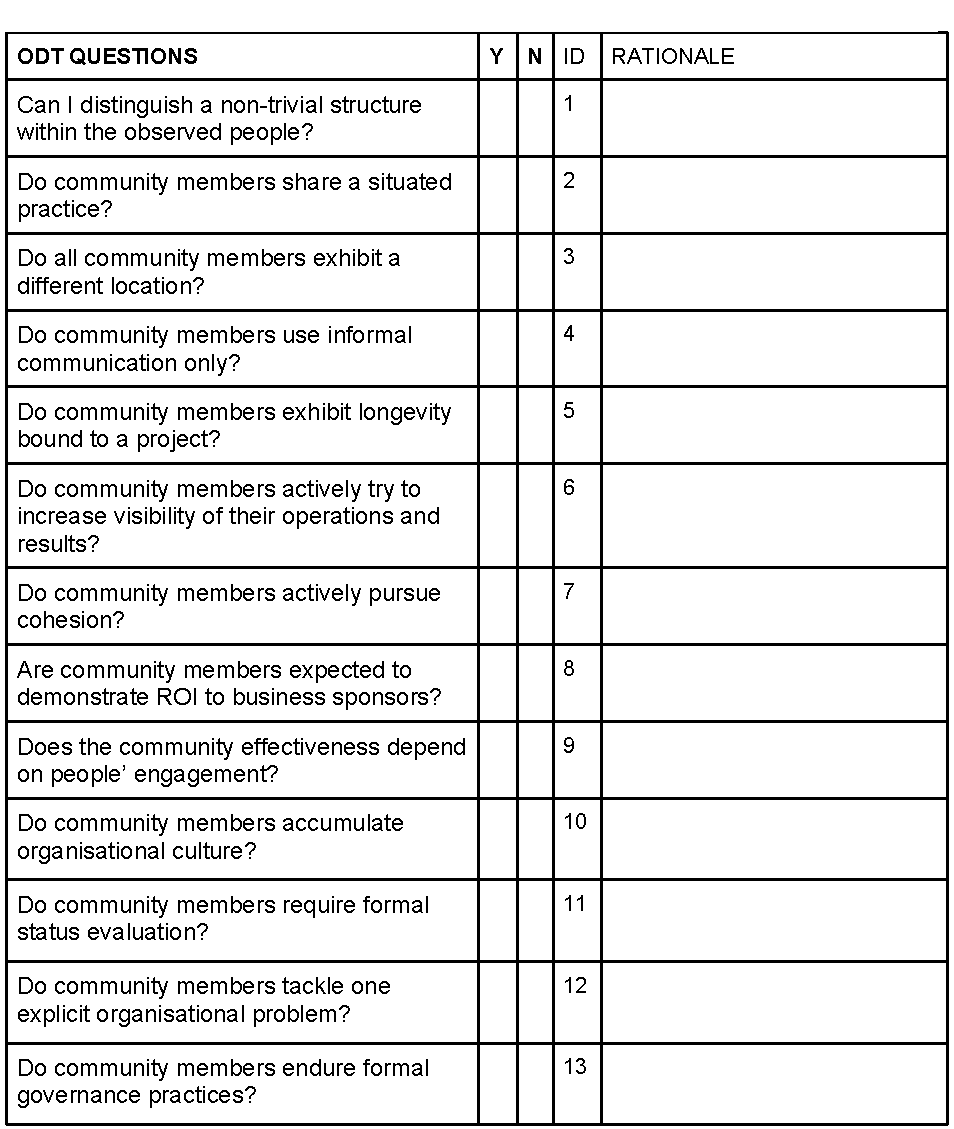
\includegraphics[width=3.5in]{quest}%
%\end{sideways}
\caption{sorting out organisational information: a questionnaire.}\label{quest}
\end{figure}
Three key sources of evidence were used:
\begin{enumerate}
\item The first key resource is a research report studying agile and open-source adoption in Company X. The study was conducted using grounded-theory \cite{gt}, to analyse interviews and artefacts alike. The study offers an overview of the organisational structure of Company X as a whole (i.e. as a global community) as well as explaining its various ``localised'' facets (i.e. in local sites). The research focuses on a division of Company X, working on a specific project release, at the time of investigation.
\item The second key resource is a research report studying three software engineering teams within Company X. The organisational details of this report focus around software process, software coding methods, development best-practices adopted, problems found, and ultimately, the people's perspective on all the above.
\item The third key resource is a set of tutorial slides that agile coaches within Company X used to introduce X's organisational structure and process to new staff.
%\item explain unique input by martin
\end{enumerate}

All of the above sources are dated around 2012. At the time of investigation, Company X was going through many organisational changes and both studies aimed at understanding the impact of organisational change on teams, their production velocity, community productivity and end-product quality. 

%\subsection{Methods}
\section{Snapshotting Communities: a Case-Study}\label{cs}

We began the case-study by analyzing the evidence available to apply the method in \cite{specissue}. The method allows associating a single community type to multiple observable attributes, through a decision-tree (see Fig. \ref{tree}). The tree however, is a single-decision mechanism that clashed with the sheer size and cluttering of organisational information from our real-life scenario. 

To dig deeper, we needed a mechanism to support the decision-tree. Consequently, we used a questionnaire to sort out the evidence available. The questionnaire is shown in Fig. \ref{quest}. The questionnaire gathers necessary organisational information, without limiting the observer's to a single path on a decision-tree. Column 1 of the questionnaire provides the (YES-NO) question that needs answering; Column 4 provides an ID for the question, to ease the mapping on the community decision-tree; finally, Column 5 requires the observer to capture the rationale of the answer, i.e. the piece of organisational information that allowed the decision.
\begin{figure}[h!]
\hspace{-.2cm}
%\begin{sideways}
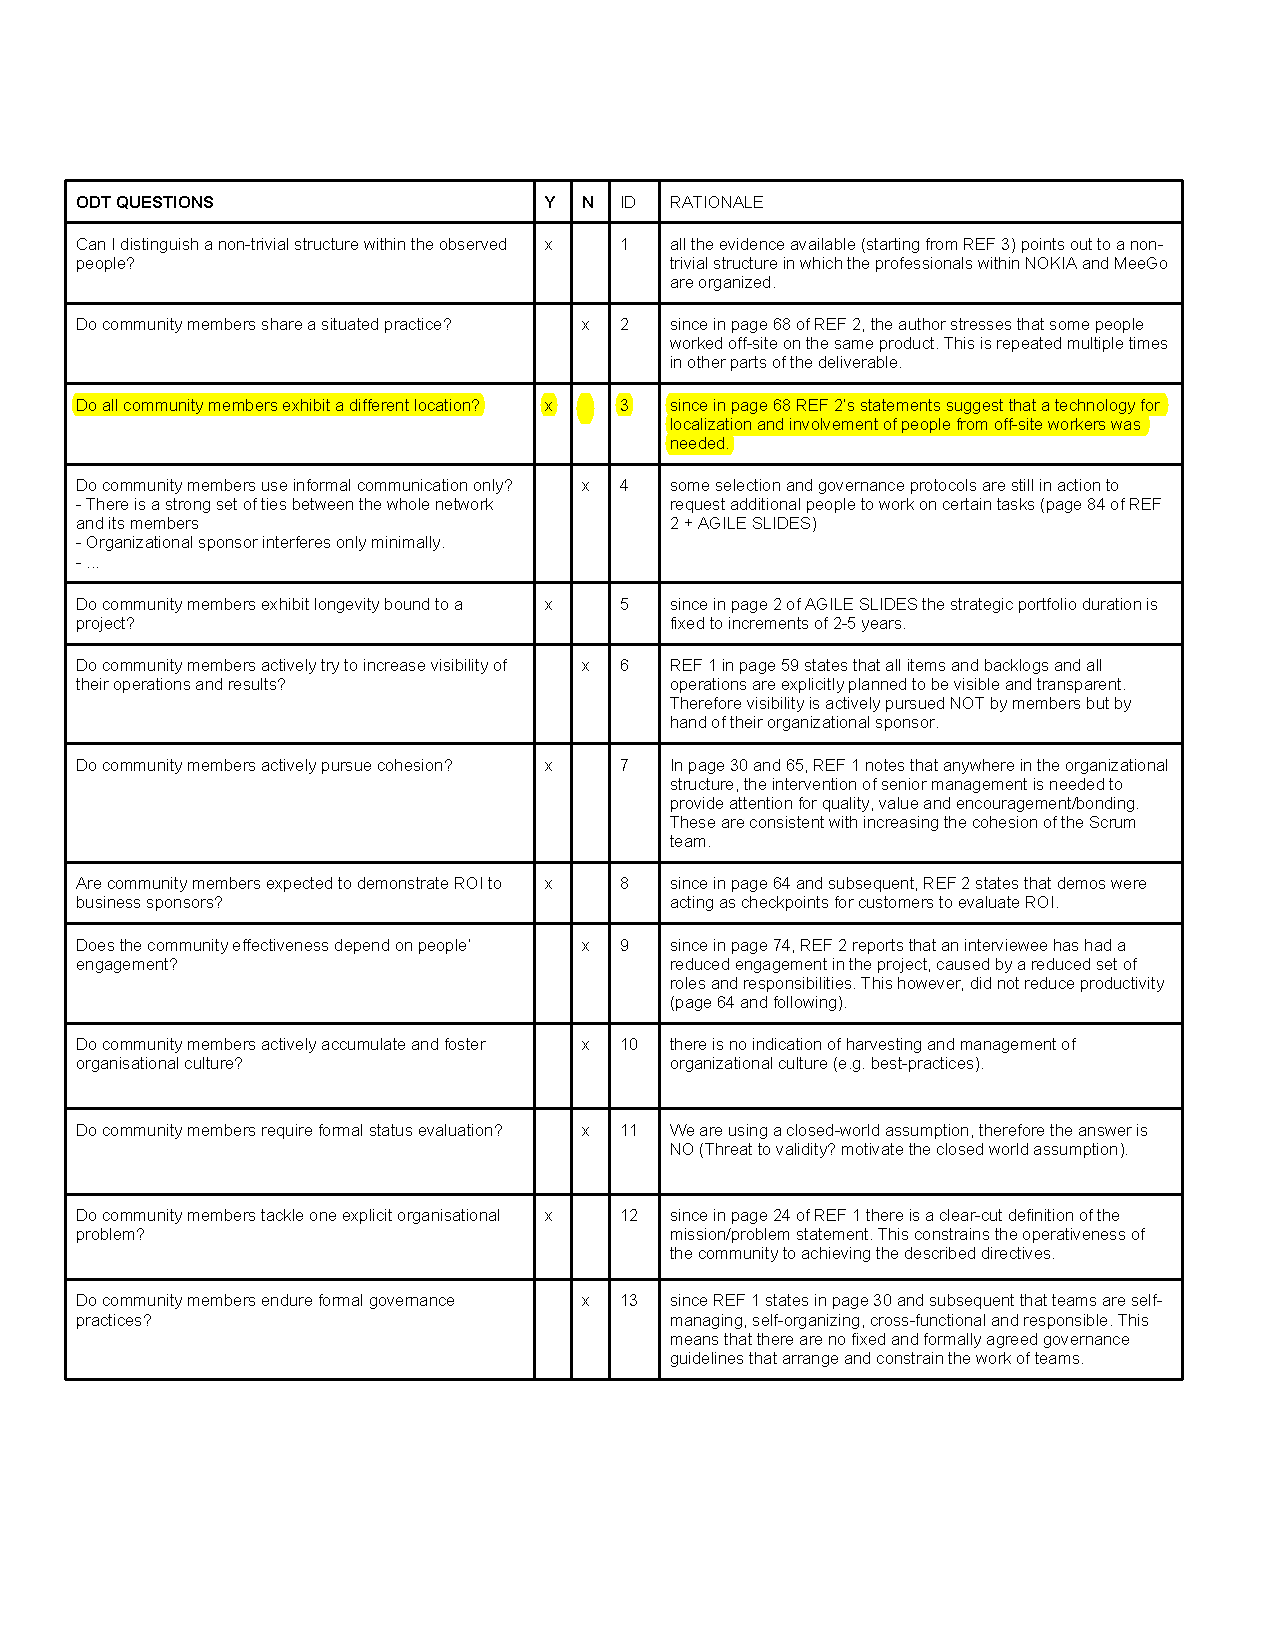
\includegraphics[width=3.5in]{answers}%
%\end{sideways}
\caption{Company X, a case-study: questionnaire with answers; in question 3, a point of indecision.}\label{answers}
\end{figure}

Based on the information available, our scenario is reflected on the questionnaire in Fig. \ref{answers}. With the empirical evidence available, we were able to clearly answer most questions except question 3: ``do all community members exhibit a different location?''. Organisational information leading to both a ``YES'' or a ``NO''. We noticed that organisational information leading to ``YES'' was related to Company X as a whole. Conversely, organisational information leading to ``NO'' was referring to only a few sites within Company X. 
%TODO: put figure of the answered questionnaire. on the figure, the pivot answers need to be with interrogation marks\\
%TODO: explain the answers\\

Once the questionnaire was completed, we matched the answers therein with the decision-tree, to identify the corresponding community types. The result of the mapping to the decision-tree is shown in Figure \ref{result}. We noticed that, when mapped to the decision-tree, the point of indecision marks the start of another path. The point of indecision acts as a \emph{pivot} around which ``revolve'' decision-tree visits.
%TODO: then proceed with showing the tree visit.\\
\begin{figure}[h!]
\hspace{-.2cm}
%\begin{sideways}
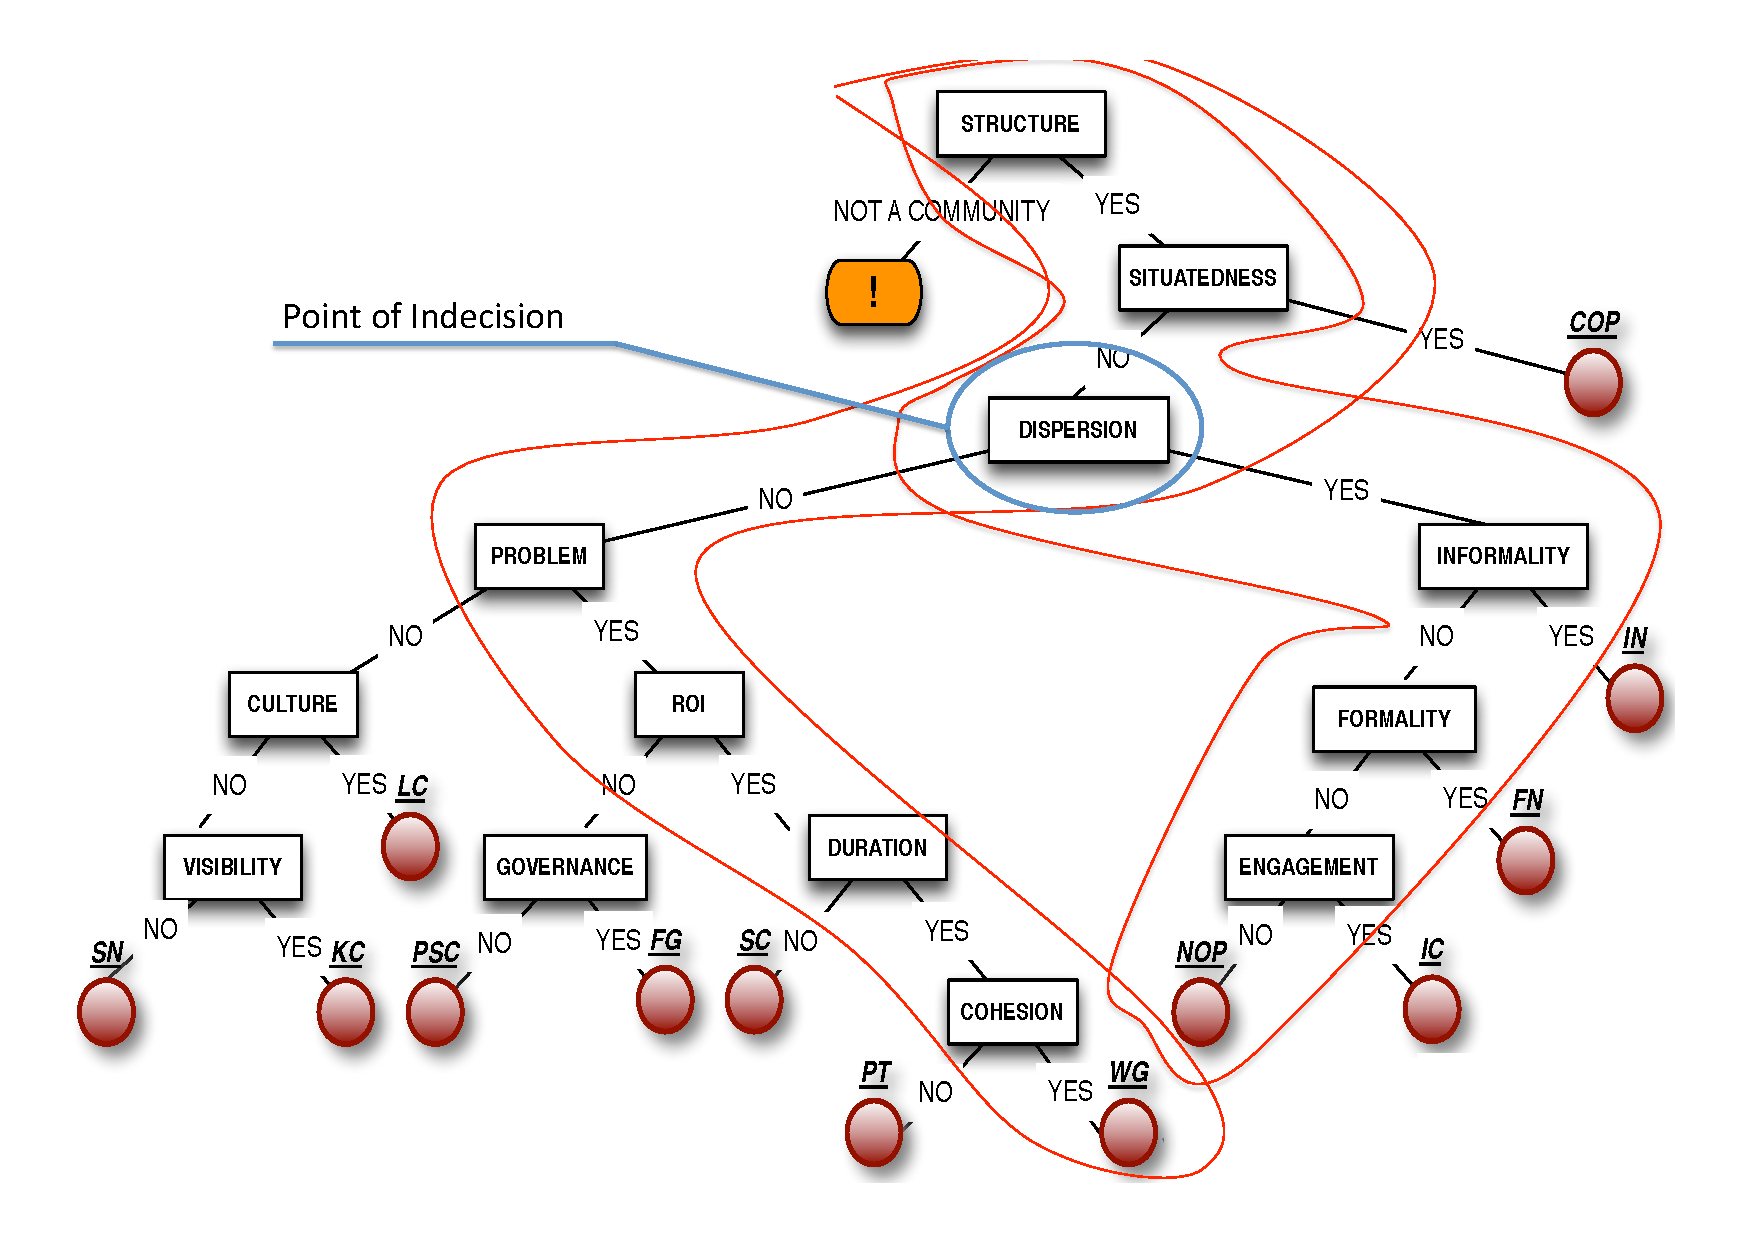
\includegraphics[width=3.5in]{visits}%
%\end{sideways}
\caption{Company X, a case-study: decision-tree visits; the point of indecision acts as a \emph{pivot} between visits.}\label{result}
\end{figure}
%\begin{itemize}
%\item explain how the case-study was conducted
%\item explain what the evidence used to give an answer to the questionnaire
%\item show the questionnaire and the visits
%\item explain types found in the case
%\item explain the design of the case-study: (a) through a questionnaire\footnote{link to URL of ODeSSATemplate.gdoc}; (b) the decision-tree described in \cite{specissue});
%\item explain the way we had to proceed in separate cases and weekly meet to share ideas and discussion of approach only limited to clarification of tasks
%\item overseeing of two senior researchers
%\end{itemize}

% An example of a floating figure using the graphicx package.
% Note that \label must occur AFTER (or within) \caption.
% For figures, \caption should occur after the \includegraphics.
% Note that IEEEtran v1.7 and later has special internal code that
% is designed to preserve the operation of \label within \caption
% even when the captionsoff option is in effect. However, because
% of issues like this, it may be the safest practice to put all your
% \label just after \caption rather than within \caption{}.
%
% Reminder: the "draftcls" or "draftclsnofoot", not "draft", class
% option should be used if it is desired that the figures are to be
% displayed while in draft mode.
%
%\begin{figure}[!t]
%\centering
%\includegraphics[width=2.5in]{myfigure}
% where an .eps filename suffix will be assumed under latex, 
% and a .pdf suffix will be assumed for pdflatex; or what has been declared
% via \DeclareGraphicsExtensions.
%\caption{Simulation Results}
%\label{fig_sim}
%\end{figure}

% Note that IEEE typically puts floats only at the top, even when this
% results in a large percentage of a column being occupied by floats.

\section{Discussion and Findings}\label{res}

An important observation we made is, that the method used during the case-study can be generalised. In addition, we made four key findings (below, in {\bf bold}). First, we found that the questionnaire has many uses other than gathering the needed organisational information. Second, we found that \emph{pivot} points can have multiple answers for the same community, this detail makes them worthy of particular attention. Third, we found that data in the questionnaire can assume five possible forms, each with some interesting properties. Fourth, organisational barriers can either be useful to shape an organisation or harmful to its operations. The text below explains all findings in more detail. In \emph{italic} we provide a discussion of the finding.

\subsection{ODeSSA: a method for Outlining Development Social Structures to Analyse}
%
%diversi usi della tabella:
%1. social communities multiple
%2. incompletezza? fungi da checklist
%3. ingegnerizzate una community per sw dev in forward
% inoltre, storia dei pivot e cosa significano
% inoltre, possibili forme e cosa significano

\subsection{Findings and Observations}

%{\bf First, we found that observable organisational information misleads the detection of communities.}
%%
%\emph{This suggests that observable organisational information is overloaded with data. A questionnaire is an essential piece to organise and contain only the necessary and sufficient information to uncover a community type. In addition, this finding also suggests that some organisational information might be missing or incomplete. The questionnaire can also be used as a checklist to make sure all needed information is actually available. Finally, this finding implies that our method for community detection cannot be fully automated.}
%TODO: make examples of each of the above statements.\\

{\bf First, the questionnaire part of the ODeSSA method� }
TODO: finish explaining\\
TODO: add example\\
TODO: explain how the finding was extracted from our case study and how and why it can be generalized\\

{\bf Second, pivots are decision-points common to all paths that describe an observable community. According to organisational information available, pivot points can be given a certain answer within one context (e.g. on a global scale) and another answer in a different context (e.g. focusing on a single site within the organisation). Stemming from this property, these decision-points represent key variations that distinguish a community from its sub-communities.}
%More in particular you need to visit the tree once per every possible combination of all \emph{pivots}.
\emph{In the status of a community, pivots are foci that differentiate the overall community type of an organisation, from the type of its constituent parts. Consequently, pivots can be used as drivers for the analysis of the community status. For example, suppose your organisational information suggests the presence of both a Formal Network (FN) and a Network-of-Practice (NoP). The pivot-point in this case is ``formality''. It follows that the community you are observing behaves formally at one level (for example on a global scale, or between sites) and informally at another level (for example between divisions or business units). It's at least something you might want to think about, if the community you are observing exhibits organisational or communication problems. Moreover, suppose you are investigating communities that should all behave in the same way. The pivot-points suggest who is diverging. You might want to consider if and why the divergence is a good thing.}
TODO: use example of pivot from case-study\\

{\bf Third, we found that the information in the ODeSSA questionnaire can assume five possible forms: (1) \emph{simple} status, represents the presence of a single path; (2) \emph{enriched-community} status, represents the presence of a path blended with attributes from other types; (3) \emph{complex} status, represents the presence of a more than one path; (4) \emph{uncertain} status, represents the presence of sparse attributes that don't represent any path but only broken segments.}
\emph{The five types can be used as a metric to evaluate community complexity. If the community matches a single path then it's more controllable, since it refers to a single type known to literature. Steering and management complexity increases the more the type diverges from simple.}
TODO: finish explaining the fifth status and elaborate on the others; make sure that they are all\\
TODO: add example\\

{\bf Finally, organisational literature defines barriers as mechanisms or circumstances that filter organisational activity \cite{Correia2010}. We found that many barriers are present in software development communities but are not necessarily a bad thing.}\\
TODO: needs the reasoning about barriers Me+Hans \\
TODO: Add example\\
%If they are, then they constrain people's communication. 
%\section{Discussion}\label{disc}

% An example of a double column floating figure using two subfigures.
% (The subfig.sty package must be loaded for this to work.)
% The subfigure \label commands are set within each subfloat command, the
% \label for the overall figure must come after \caption.
% \hfil must be used as a separator to get equal spacing.
% The subfigure.sty package works much the same way, except \subfigure is
% used instead of \subfloat.
%
%\begin{figure*}[!t]
%\centerline{\subfloat[Case I]\includegraphics[width=2.5in]{subfigcase1}%
%\label{fig_first_case}}
%\hfil
%\subfloat[Case II]{\includegraphics[width=2.5in]{subfigcase2}%
%\label{fig_second_case}}}
%\caption{Simulation results}
%\label{fig_sim}
%\end{figure*}
%
% Note that often IEEE papers with subfigures do not employ subfigure
% captions (using the optional argument to \subfloat), but instead will
% reference/describe all of them (a), (b), etc., within the main caption.


% An example of a floating table. Note that, for IEEE style tables, the 
% \caption command should come BEFORE the table. Table text will default to
% \footnotesize as IEEE normally uses this smaller font for tables.
% The \label must come after \caption as always.
%
%\begin{table}[!t]
%% increase table row spacing, adjust to taste
%\renewcommand{\arraystretch}{1.3}
% if using array.sty, it might be a good idea to tweak the value of
% \extrarowheight as needed to properly center the text within the cells
%\caption{An Example of a Table}
%\label{table_example}
%\centering
%% Some packages, such as MDW tools, offer better commands for making tables
%% than the plain LaTeX2e tabular which is used here.
%\begin{tabular}{|c||c|}
%\hline
%One & Two\\
%\hline
%Three & Four\\
%\hline
%\end{tabular}
%\end{table}


% Note that IEEE does not put floats in the very first column - or typically
% anywhere on the first page for that matter. Also, in-text middle ("here")
% positioning is not used. Most IEEE journals/conferences use top floats
% exclusively. Note that, LaTeX2e, unlike IEEE journals/conferences, places
% footnotes above bottom floats. This can be corrected via the \fnbelowfloat
% command of the stfloats package.

\section{Threats to Validity}
\begin{itemize}
\item minna and ossi are two different situations in two different points in time. results confirmed by executing the case-study twice, contemporarily by two different researchers.
\item observations are made on only a single case-study.
\end{itemize}

\section{Conclusion and Future Work}\label{conc}

TODO: explain possible followup studies, connected to the notion of community snapshot.\\
% conference papers do not normally have an appendix

% use section* for acknowledgement
\section*{Acknowledgment}

The authors would like to thank beer, Mrs. Mirella Sangiovanni's home-made sweets and her mother's home-made cheese.

% trigger a \newpage just before the given reference
% number - used to balance the columns on the last page
% adjust value as needed - may need to be readjusted if
% the document is modified later
%\IEEEtriggeratref{8}
% The "triggered" command can be changed if desired:
%\IEEEtriggercmd{\enlargethispage{-5in}}
% references section

% can use a bibliography generated by BibTeX as a .bbl file
% BibTeX documentation can be easily obtained at:
% http://www.ctan.org/tex-archive/biblio/bibtex/contrib/doc/
% The IEEEtran BibTeX style support page is at:
% http://www.michaelshell.org/tex/ieeetran/bibtex/
\bibliographystyle{IEEEtran}
% argument is your BibTeX string definitions and bibliography database(s)
\bibliography{community}
%
% <OR> manually copy in the resultant .bbl file
% set second argument of \begin to the number of references
% (used to reserve space for the reference number labels box)
%\begin{thebibliography}{1}
%
%\bibitem{IEEEhowto:kopka}
%H.~Kopka and P.~W. Daly, \emph{A Guide to \LaTeX}, 3rd~ed.\hskip 1em plus
%  0.5em minus 0.4em\relax Harlow, England: Addison-Wesley, 1999.
%
%\end{thebibliography}




% that's all folks
\end{document}


